\documentclass[landscape,final,a0paper,fontscale=0.285]{baposter}

\usepackage{calc}
\usepackage{graphicx}
\usepackage{amsmath}
\usepackage{amssymb}
\usepackage{relsize}
\usepackage{multirow}
\usepackage{rotating}
\usepackage{bm}
\usepackage{url}

\usepackage{graphicx}
\usepackage{multicol}


%\usepackage{times}
%\usepackage{helvet}
%\usepackage{bookman}
\usepackage{palatino}
%\usepackage{arial}

\newcommand{\captionfont}{\footnotesize}

\graphicspath{{images/}{../images/}}
\usetikzlibrary{calc}

\newcommand{\SET}[1]  {\ensuremath{\mathcal{#1}}}
\newcommand{\MAT}[1]  {\ensuremath{\boldsymbol{#1}}}
\newcommand{\VEC}[1]  {\ensuremath{\boldsymbol{#1}}}
\newcommand{\Video}{\SET{V}}
\newcommand{\video}{\VEC{f}}
\newcommand{\track}{x}
\newcommand{\Track}{\SET T}
\newcommand{\LMs}{\SET L}
\newcommand{\lm}{l}
\newcommand{\PosE}{\SET P}
\newcommand{\posE}{\VEC p}
\newcommand{\negE}{\VEC n}
\newcommand{\NegE}{\SET N}
\newcommand{\Occluded}{\SET O}
\newcommand{\occluded}{o}

%%%%%%%%%%%%%%%%%%%%%%%%%%%%%%%%%%%%%%%%%%%%%%%%%%%%%%%%%%%%%%%%%%%%%%%%%%%%%%%%
% Multicol Settings
%%%%%%%%%%%%%%%%%%%%%%%%%%%%%%%%%%%%%%%%%%%%%%%%%%%%%%%%%%%%%%%%%%%%%%%%%%%%%%%%
\setlength{\columnsep}{1.5em}
\setlength{\columnseprule}{0mm}

\newcommand{\compresslist}{%
\setlength{\itemsep}{1pt}%
\setlength{\parskip}{0pt}%
\setlength{\parsep}{0pt}%
}

\begin{document}

% Define some colors

\definecolor{lightblue}{cmyk}{0.83,0.24,0,0.12}
\definecolor{lightblue}{rgb}{.1,.43,.14}

\begin{poster}%
  % Poster Options
  {
  % Show grid to help with alignment
  grid=false,
  % Column spacing
  colspacing=1em,
  % Color style
  bgColorOne=white,
  bgColorTwo=white,
  borderColor=black,
  headerColorOne=lightblue,
  headerColorTwo=lightblue,
  headerFontColor=white,
  boxColorOne=white,
  boxColorTwo=lightblue,
  % Format of textbox
  textborder=roundedleft,
  % Format of text header
  eyecatcher=true,
  headerborder=closed,
  headerheight=0.1\textheight,
  textfont=\sc, %An example of changing the text font
  headershape=roundedright,
  headershade=shadelr,
  headerfont=\Large\bf\textsc, %Sans Serif
  textfont={\setlength{\parindent}{1.5em}},
  boxshade=plain,
%  background=shade-tb,
  background=plain,
  linewidth=2pt
  }
  % Eye Catcher
  {
\includegraphics[height=6em]{img/Clarkson}} 
  % Title
  {\bf\textsc{Nondimensionalizing a System of Differential Equations}\vspace{0.5em}}
  % Authors
  {\textsc{Amanda Groccia, Tatyania Moorehead, Carrie Rider}}
  % University logo
  {% The makebox allows the title to flow into the logo, this is a hack because of the L shaped logo.

\includegraphics[height=6.0em]{img/Clarkson}
  }


%%%%%%%%%%%%%%%%%%%%%%%%%%%%%%%%%%%%%%%%%%%%%%%%%%%%%%%%%%%%%%%%%%%%%%%%%%%%%%
  \headerbox{Background}{name=definition,column=0,row=0}{

Nondimensionalization is a method used to scale problems in order to analyze the behavior of a system regardless of the units used. The motivation behind this method is to reduce the number of parameters in a given system of equations.


}
% % % % % % % % % % % % % % % % % % % % % % % % % % % % % % % % % % % % % %

 \headerbox{Process}{name=solve,column=0,below=definition}{
\begin{center}

\begin{enumerate}
\item
	List all the variables and parameters along with their dimensions.
	
\item
	For each variable, say $x$, form a product (or quotient) $p$ of parameters that has the same dimensions as $x$, and define a new variable $y=\frac{x}{p}.$ $y$ is a "dimensionless" variable. It's numerical  value is the same no matter what system of units is used.
	
\item Rewrite the differential equation in terms of the new variables.

\item 
	Group the parameters into nondimensional combinations, and define a new set of nondimensional parameters expressed as the nondimensional combinations of the original parameters.
	 
\end{enumerate}
\end{center}
}
% % % % % % % % % % % % % % % % % % % % % % % % % % % % % % % % % % % % %
  \headerbox{Logistic Equation}{name=definition,column=0,below=solve}{
  
A fundamental example is the Logistic Equation: 
    $$\frac{dx}{dt} = rx \left(1-\frac{x}{K}\right), \hspace{.25em} x(0)=x_0$$

  
To nondimensionalize this problem the following substitutions are made:
\begin{align*}
		& x \rightarrow A \hat{x} (s) \\
		& y \rightarrow B \hat{y} (s) \\
		& t \rightarrow \tau \cdot s
\end{align*}
After making the following substitutions,

		$$A = K, \hspace{.5em}
		\tau = \frac{1}{r},$$
the nondimensionalized system is $$\frac{d{x}}{dt}= x(1-x), \hspace{.25em} x(0)=x_0.$$


}
%%%%%%%%%%%%%%%%%%%%%%%%%%%%%%%%%%%%%%%%%%%%%%%%%%%%%%%%%%%%%%%%%%%%%%%%%%%%%%
  \headerbox{Discussion}{name=simple,column=1,row=0}{

Based on the nondimensionalization of the logistic model it is clear that the parameters do not affect the overall behavior of the system. Only the initial condition affects the basic trends. 

\begin{center}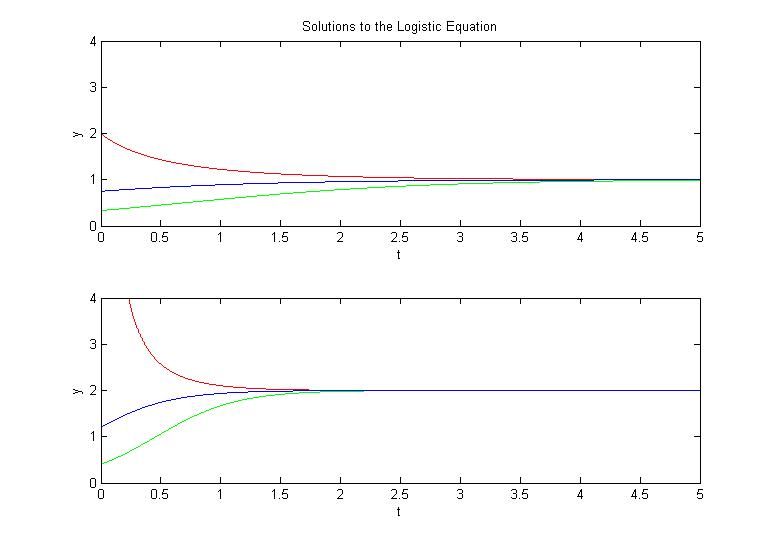
\includegraphics[width=7.5cm,height=7cm]{img/ScalingofLogisticEqn} \end{center}

The plots above show various solutions to the logistic equation with different initial conditions (represented by different color) and scaling.  From these plots we can see that the overall behavior is the same with all conditions converging to a stable equilibrium solution. The scaling of time and height is different, but does not change the basic behavior. 
}
% % % % % % % % % % % % % % % % % % % % % % % % % % % % % % % % % % % %
\headerbox{Buckingham-Pi Theorem}{name=graphs,column=1,below=simple}{
%\centering
%\hspace*{-.5cm}
%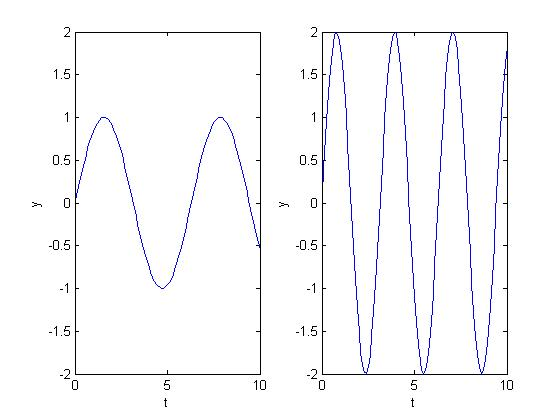
\includegraphics[width=5cm]{img/ScaledPlots}
%\begin{center}Figure 1: Differently scaled sine functions.  \end{center}

\flushleft
\textbf{The Buckingham Pi Theorem} is a scheme for nondimensionalization. The theorem states if $q_1,q_2,q_3, \cdots, q_n$ are $n$ dimensional variables that are physically relevent in a given problem that are inter-related by a dimensionally homogeneous set of equations. They can be expressed via a functional relationship of the form: 
$$F(q_1,q_2,\cdots, q_n)=0 \hspace{.5em}$$ 
or equivalently
$$q_1=f(q_2, \cdots, q_n).$$ 
 }
% % % % % % % % % % % % % % % % % % % % % % % % % % % % % % % % % % % % %
\headerbox{Killer Shrimp}{name=killershrimp,column=2,row=0}
{
Southern German water routes have had several drastic population
changes concerning gammarids (Kinzler, 2008). Much of this is due to canal construction.

 Of the five species who have lived in these waters, \textit{Dikerogammarus villosus (Dv)}, denoted $x$, and \textit{Dikerogammarus haemobaphes (Dh)}, denoted $y$, are the two dominating species.

\begin{center}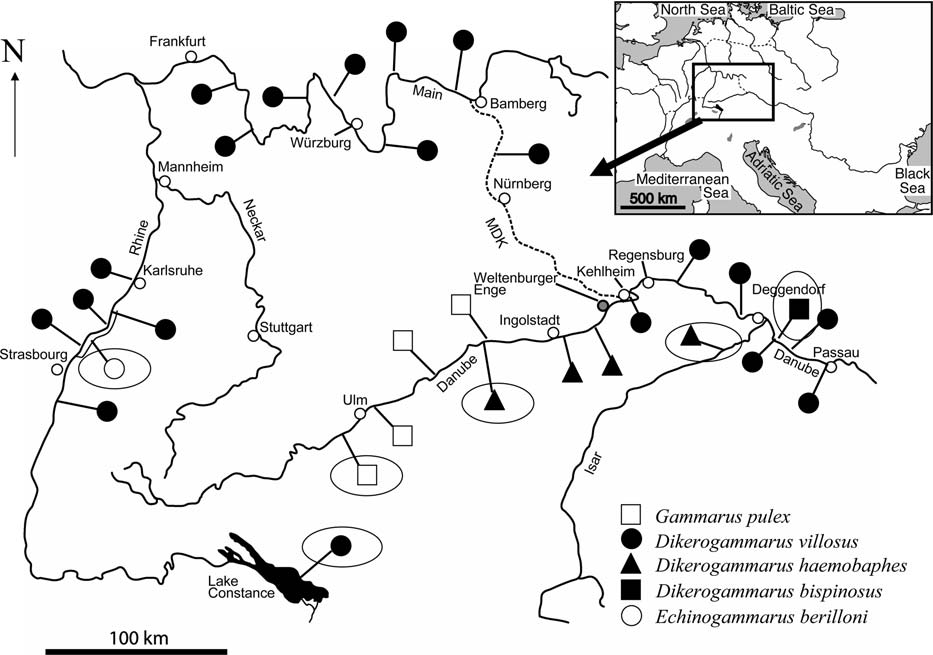
\includegraphics[width=7.5cm,height=7cm]{img/kinzlermap} 
Figure: A map of gammarid populations in the Southern German waters. (Kinzler, 2008) \end{center}

Due to the position of gammarids, or shrimp, on the food chain, they play a vital role in the ecological conditions of their environment. That is, if their populations experience a major change the ecology of the entire area may shift. 

One characteristic of the shrimp in this area is that they prey on other shrimp of other species as well as their own kind (cannibalism). This means the populations of each species have a strong interdependancy. 

}

%%%%%%%%%%%%%%%%%%%%%%%%%%%%%%%%%%%%%%%%%%%%%%%%%%%%%%%%%%%%%%%%%%%%%%%%%%%%%%
\headerbox{Mutual Predation Example}{name=history,column=3,row=0}
{
The two populations can be modeled by:
   \begin{align*}
    \frac{dx}{dt} & = rx^2 \left(1-\frac{x}{K}\right) - \alpha xy - \frac{x^2 \gamma_\circ}{x+D}, \\
    \frac{dy}{dt} & = \rho y^2 \left(1-\frac{y}{L}\right) - \beta xy -\frac{y^2 \delta_\circ}{y+R}.
  \end{align*}
  The intraguild predation is proportional to $$xy.$$
  The canabalism for species $x$ is proportional to $$\frac{x^2}{x+D}.$$
  The canabalism for species $y$ is proportional to $$\frac{y^2}{y+R}.$$ 
	
}

%%%%%%%%%%%%%%%%%%%%%%%%%%%%%%%%%%%%%%%%%%%%%%%%%%%%%%%%%%%%%%%%%%%%%%%%%%%%%%
  \headerbox{Mutual Predation Solution} {name=Zombie,column=3,span=1, below=history}{
    The model becomes
        \begin{align*}
            \frac{dx}{dt} & = x^2 (1-x) - \frac{\alpha L}{rK} xy - \frac{\frac{1}{rK}x^2 \gamma_\circ}{x + \frac{D}{K}} \\
            \frac{dy}{dt} & = \frac{\rho L}{rK} y^2 (1-y) - \frac{\beta}{r} xy - \frac{\frac{1}{rK}y^2 \delta_\circ}{y + \frac{R}{L}}.
        \end{align*} 
        The substitutions are
        $$A=K, \hspace{.2em} B=L,\hspace{.2em} and \hspace{.2em} \tau=\frac{1}{rK}.$$%\\ [3pt]
       The nondimensionalized system is
    $$\frac{dx}{dt} = x^2 (1-x) - \alpha xy - \frac{\gamma_\circ x^2}{x+D},$$
    $$\frac{dy}{dt} = \rho y^2 (1-y) - \beta xy -\frac{\delta_\circ y^2}{y+R}.$$
 }

%%%%%%%%%%%%%%%%%%%%%%%%%%%%%%%%%%%%%%%%%%%%%%%%%%%%%%%%%%%%%%%%%%%%%%%%%%%%%%

%%%%%%%%%%%%%%%%%%%%%%%%%%%%%%%%%%%%%%%%%%%%%%%%%%%%%%%%%%%%%%%%%%%%%%%%%%%%%%
 

%%%%%%%%%%%%%%%%%%%%%%%%%%%%%%%%%%%%%%%%%%%%%%%%%%%%%%%%%%%%%%%%%%%%%%%%%%%%%%


%%%%%%%%%%%%%%%%%%%%%%%%%%%%%%%%%%%%%%%%%%%%%%%%%%%%%%%%%%%%%%%%%%%%%%%%%%%%%%%
%\headerbox{Future Research}{name=app, column=3, below=graphs}{
%For the future, multivariate sensitivity should be examined and the initial value of $M$ could be explored as it could be a value that %is too big.
%}

%%%%%%%%%%%%%%%%%%%%%%%%%%%%%%%%%%%%%%%%%%%%%%%%%%%%%%%%%%%%%%%%%%%
\headerbox{Acknowledgments}{name=ref,column=3,above=bottom}{
Thanks to Dr. Joel Foisy, Dr. Kelly Black, The NSF (DSM-1262737) and
The NSA (H98230-14-1-0141) for their support. 
%\smaller
%\bibliographystyle{ieee}
%\renewcommand{\section}[2]{\vskip 0.05em}
%\begin{thebibliography}{1}\itemsep=-0.01em
%\setlength{\baselineskip}{0.4em}
%\bibitem{biology}
%\url{http://www.plosbiology.org/article/info}
%\bibitem{reproductive}
%\url{http://www.ganfyd.org/index.php?title=Reproductive_number}
%\end{thebibliography}
%\vspace{0.3em}
}


%%%%%%%%%%%%%%%%%%%%%%%%%%%%%%%%%%%%%%%%%%%%%%%%%%%%%%%%%%%%%%%%%%%
\headerbox{Conclusion}{name=infections,column=2,above=bottom}{
Nondimsionalization is a very useful and convenient method for optimizing the efficiency of experiments. This is because we can recognize whether the parameters themselves matter, the ratios of the parameters, or if they don't matter at all. 
}
\end{poster}

\end{document}
